\section{Introduction}
Supporting the workflow of a surgeon can be a tricky thing.
By studying the workflow of a orthopedic surgeon during a scoliosis surgery Pedersson et. al.\cite{Pederson:2015} discovered multiple challenges which need to be overcome to support the workflow of such professionals.

First there exists an issue that the information sharing between different departments provides some information technological  challenges due to spatial issues.
Departments such as laboratories, radiology and the like are spread all over the hospital rather than all being located at one spot.
Additionally information ready at hand for when visiting patients in the hopsital wards is of high relevance to the physician. 

Another observation which is made is the fact that the personel use multiple screens to present data.
This is due to the fact that sterilizing computers and their periphials during surgery is difficult to do.

Hence issues such as information sharing, presentation of multiple data feeds and interaction without contamination of periphials are some of the problems discovered(for a full list of challenges please refer to figure \ref{fig:problem}).

\begin{figure}[h]
\centering
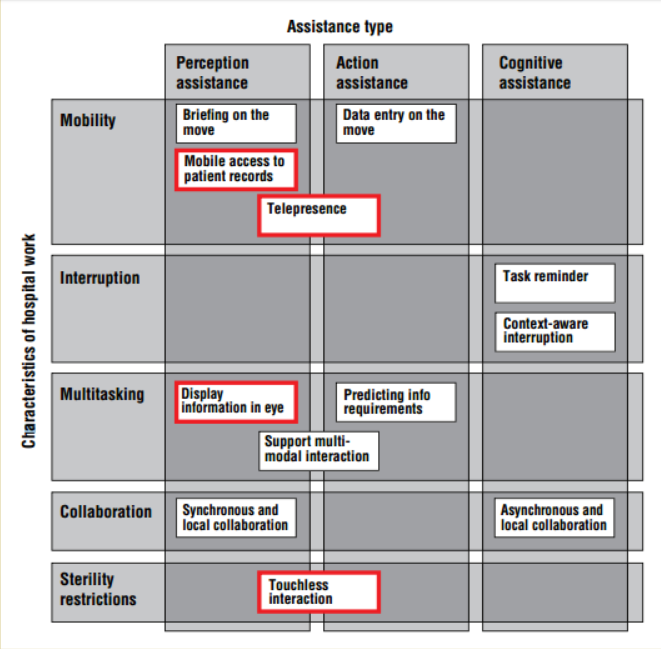
\includegraphics[width=1\columnwidth]{img/problem_areas}
\caption{A diagram depicting the issues discovered by the ethnographic study performed by Pederson et. al. }
\label{fig:problem}
\end{figure}

The system that is described in this paper aims to resolve some of the problems encountered in the previous scenarios.

The system which has been designed is able to interpret hand movements thanks to a prototype wristband. This information is the used to recognize specific movements, ultimately navigating images on an android device.

In particular, movements such as swiping the hand to the left, right, up and down are used to navigate the image,
while rotations of the wrist to the left and to the right are interpreted as zoom commands.
